\chapter{Implementation}
\index{Implementation%
@\emph{Implementation}}%

\section{Layout and Structure}
\label{sec:layout}

Speakur\index{Speakur} is delivered as a single Custom Element\index{Custom Elements}, \tcode{<speakur-discussion>}\index{<speakur-discussion>}.
You must import the tag with \tcode{<link rel=import href=...>} to make it available to place on the page. 
This element has a data-bound\index{data-bound template} \tcode{<template>}\index{<template>} that provides the element's visual representation (shadow DOM).
Actually, a custom element's representation, or logical DOM\index{Logical DOM}, may consist of both encapsulated shadow DOM\index{Shadow DOM} as well as light DOM\index{Light DOM} that is supplied by the \textit{user} of the custom element and \textit{projected} into the shadow DOM as discussed in section~\ref{bg:shadowdom}.
In the case of Speakur, the discussion forum is self-contained in terms of content; light DOM is not needed or used in the top-level element.
Speakur's\index{Speakur} options or parameters are controlled with attributes\index{HTML!attributes}:

\begin{lstlisting}[language=HTML5,caption=
{Using HTML attributes to set Speakur options},label=l:options1,captionpos=below]
 <speakur-discussion
   firebaseLocation="https://speakur-demo.firebaseio.com"
   xtitle="This is the thread's (initial) title."
   href="demo1"
   initiallyOpen="true"
   allowAnonymous="true">
 </speakur-discussion>
\end{lstlisting}

Structurally, Speakur\index{Speakur} consists of JavaScript\index{JavaScript}, HTML, and CSS\index{CSS} files, along with a few other resource types like images and JSON\index{JSON} language files. 
All of the these internal resources and components are hidden from consumers who only have to import and place the main \tcode{<speakur-discussion>}\index{<speakur-discussion>} element as discussed in section~\ref{publishing} below.
The rest of the components are brought in by imports inside \tcode{<speakur-discussion>}\index{<speakur-discussion>}.

\begin{table}\centering
\ra{1.3}
\begin{tabular}{@{}lp{8cm}@{}}
\toprule
Name & Function \\
\midrule
$Structural~containers$\\
\tcode{<speakur-discussion>} & Top-level public component. \\
\tcode{<speakur-thread-view>} & Container for the comments displayed in an entire thread. \\
\tcode{<speakur-card>} & Provides a Material Design\index{Material Design} `card' container. \\
\tcode{<speakur-post-set>} & A container for a list of posts such as replies to a specific post. \\
\\
$Logical~services$\\
\tcode{<firebase-element>}\index{<firebase-element>} & Web Component wrapper around Firebase\index{Firebase}. \\
\tcode{<speakur-base>} & Base-class for most other Speakur components. \\
\tcode{<speakur-i18next>} & WC wrapper around i18next library. \\
\tcode{<speakur-profile>} & Users' session data and preferences. \\
\tcode{<speakur-post-vote>} & Controller for voting posts up or down. \\
\\
$User~Interface$\\
\tcode{<speakur-compose>} & Composing replies and posts. \\
\tcode{<speakur-post>} & Displays a single user post/comment. \\
\tcode{<speakur-login-button>} & Login/logout button and dropdown. \\
\tcode{<speakur-theme>} & Base class for all themes, mainly CSS rules. \\
\tcode{<speakur-theme-blue>} & A specific theme. \\
\tcode{<speakur-dialog-profile>} & Dialog to edit user preferences. \\
\tcode{<speakur-lang-select>} & Dropdown to choose the UI language. \\
\bottomrule
\end{tabular}
\caption{A partial list of Speakur's internal components.}
\label{table:speakurcomponents}
\end{table}

Internally, Speakur\index{Speakur} is composed of a number of sub-components, a partial list of which is found in table~\ref{table:speakurcomponents}. 
These components are listed in three broad categories: structural containers, 
logical services, 
and user interface\index{user interface (UI)} elements.
The structural elements provide a container and abstraction layer for a group of related child elements, such as \tcode{<speakur-card>}, 
which provides a Material Design-styled\index{Material Design} `card' consisting of a header, body, and footer.
These containers may have certain visible elements such as lines around the border, but most of their representation comes from the components inside.

The logical service elements do not have any visual representation at all.
They perform data-related services, provide purely abstract APIs, and wrap external libraries.
For example, the Firebase\index{Firebase} client library is a general purpose JavaScript library, and is not specifically adapted to Web Components or custom elements.
Therefore it is often useful to provide a custom element wrapper around a non-WC-aware library.
For this reason the Polymer project maintains \tcode{<firebase-element>}\index{<firebase-element>} as a wrapper around the main Firebase library~\cite{polymercontributors2015-c}.
Within Speakur, each component gets its data either directly from its own internal \tcode{<firebase-element>}\index{<firebase-element>}, or else from a data binding from a parent element that it got from its own \tcode{<firebase-element>}\index{<firebase-element>}.

Figure~\ref{f:file_layout} shows a partial listing of the internal component files.
One of these is abstraction layer for an internationalization\index{internationalization} library.
Following the \tcode{<firebase-element>}\index{<firebase-element>} example, 
I created a simple custom element wrapper around the \textbf{i18next} 
JavaScript\index{JavaScript} library~\cite{i18nextcontributors2015}.
This wrapper is called \tcode{<speakur-i18next>}\index{<speakur-i18next>}. 
It tells i18next where to find Speakur's translation files and creates a Polymer \textit{expression} to perform translations from data-bound templates. 
See section~\ref{sec:i18n} below for details.
Logical elements are also used to provide abstract `controllers' 
(in the MVC\index{model-view-controller} sense), 
facades, pseudo-OOP\index{object oriented programming (OOP)} base classes and other design patterns.

\begin{figure}[htb]
	\centerline{
	\begin{subfigure}[b]{0.48\textwidth}
		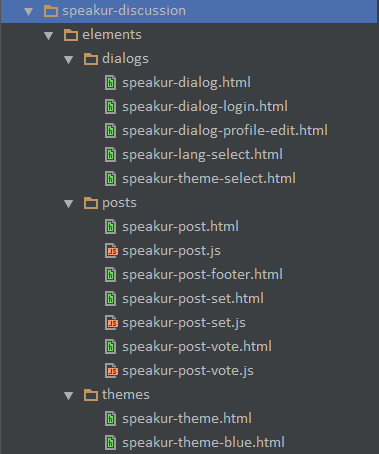
\includegraphics[width=\textwidth]{images/file_layout_a.png}
	\end{subfigure} %
	\begin{subfigure}[b]{0.48\textwidth}
		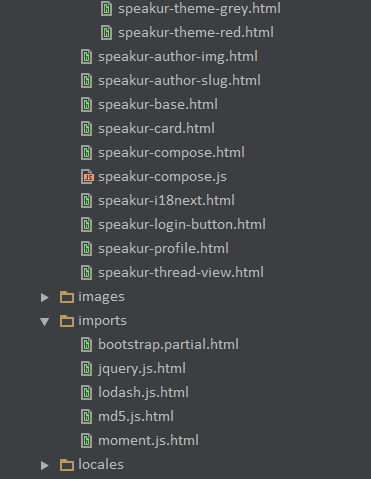
\includegraphics[width=\textwidth]{images/file_layout_b.png}
	\end{subfigure} %
	}
	\caption{Internal elements file layout (partial).}
	\label{f:file_layout}
\end{figure}

In addition to structural and logical elements, Speakur has a number of user interface (UI)\index{user interface (UI)} custom elements to do things like display an individual user post or show the post composition editor.
Some of these, like \tcode{<speakur-theme>}, are also `base classes' for other elements,
in a way that is similar but not identical to classes in object oriented programming (OOP)\index{object oriented programming (OOP)}\footnote{Note that JavaScript\index{JavaScript} itself is \textit{prototype}-based\index{prototype \textit{(JavaScript)}} and does not have traditional classes or inheritance. 
Similar behavior is obtained by using regular object instances (instead of classes) as the prototype for instantiating new objects.}. 
Although composition or \textit{has-a} relationships are generally preferred, inheritance or \textit{is-a} relationships can make sense when you truly want to be able to substitute one instance for another.

\section{Database Design}
\label{sec:database}

Speakur uses Firebase for NoSQL\index{NoSQL}-style database storage.
Traditional relational databases\index{relational database} (SQL\index{SQL}) have emphasized data normalization\index{normalization} -- the removal of informational redundancies from databases such that a given \textit{fact} is only recorded in a single place.
While this helps ensure data integrity, it can adversely affect query time and scalability as additional joins are required to bring in the necessary facts.
One of the defining characteristics of the NoSQL movement is denormalization\index{denormalization}
--- that is, the principle of eliminating redundancy is sacrificed in order to gain performance~\cite{sadalage2012}.
Facts can be defined in more than one place to speed up queries.

For example, in Speakur\index{Speakur}, some information about a post's author 
such as their public username, id, and photo url is saved inside each post they write 
so that it's not necessary to look up this information separately just to display the post.
One consequence of this is that changing your public name doesn't retroactively change the name on all of your previous posts, just new posts going forward.
Certainly, if that name updating was deemed necessary per business requirements, it could be accomplished.

% p{8cm}
\begin{table}\centering
\ra{1.3}
\begin{tabular}{@{}lll@{}}
\toprule
Table Name & Function & Key Structure \\
\midrule
\tcode{admins} & Administrator authorizations & \tcode{\$uid} \\
\tcode{posts} & User posts & \tcode{\$parent->\$child} \\
\tcode{postvotes} & Public vote counts for posts & \tcode{\$parent->\$child} \\
\tcode{profile} & User data and preferences & \tcode{\$uid} \\
\tcode{threads} & Discussion thread definitions & \tcode{\$threadId} \\
\tcode{uservotes} & User votes for posts & \tcode{\$uid->\$parent->\$child} \\
\bottomrule
\end{tabular}
\caption{Speakur's database tables.}
\label{table:speakurtables}
\end{table}

The logical interface presented by Firebase\index{Firebase} resembles a single JavaScript\index{JavaScript} object which can contain other objects nested up to 32 levels deep~\cite{firebasecontributors2015}.
A JavaScript object is fundamentally a \tcode{key->value} mapping, also known as a hash map or (in Python\index{Python language}) as a dictionary.
Although this nested object structure doesn't correspond exactly to traditional relational database\index{relational database} (SQL\index{SQL}) tables, 
it is convenient to refer to the top (first) level of nested objects as ``tables''.
The leaf node objects are ``records'' with data fields, and the intermediate objects are keys within the table.
Like most NoSQL databases, Firebase is forgiving with regard to structure and fields; 
a given record is not guaranteed to follow any particular structure unless this is required by the security and validation rules.

\begin{figure}[htb]
\centering
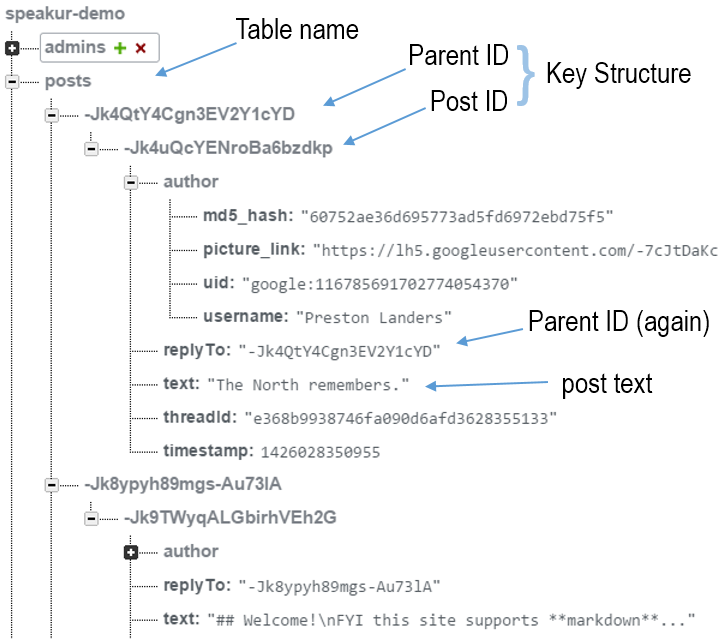
\includegraphics[width=\textwidth]{images/firebase_admin_posts_b.png}
\caption{Structure of the \tcode{posts} table.}
\label{f:firebase_admin_posts}
\end{figure}

The key structure column in table~\ref{table:speakurtables} signifies the meaning of the keys underneath a table. 
For example, the main \tcode{posts} table has a \tcode{\$parent->\$child} key structure, 
which means that the first layer of keys beneath \tcode{posts} are post \textit{parent} ids, 
meaning the id of the post that this post is a reply to, 
or the thread id in the case of a `top-level' post.
The next nested object down is the \textit{child} id, 
or the id of the actual post itself, 
and the keys under that are the `fields' of the table, 
such as the \tcode{text} and \tcode{replyTo} values.
Figure~\ref{f:firebase_admin_posts} shows Firebase's administrative view of the database where the \tcode{posts} table is expanded, 
showing the parent and child id layers, 
and the actual post nested within.
Deeply nested data structures are not good for scalability; 
relatively flat tables are best.
The key structure will become important when we apply security rules in section~\ref{sec:security}.

In addition to denormalizing\index{denormalization} the data as necessary, sometimes it is convenient for security reasons to 
keep related bits of data in separate tables in order to apply different security rules.
For instance, we want users to be able to modify a post's vote count without being able to modify the post itself.
The nested and denormalized structure of the tables helps ensure that we only fetch what we need, when we need it.
The flip side is that we need to be aware of these data duplications and update them as necessary, 
which can be difficult in a more sophisticated application.

\section{Synchronization}
\label{sec:sync}

Speakur\index{Speakur} consists of a number of Polymer components which break down the problem of presenting a discussion forum into smaller tasks.
Some of these components are listed in table~\ref{table:speakurcomponents}.
They form a hierarchy with <speakur-discussion> at the top (root). 
Figure~\ref{f:component_layout} illustrates this, with many components omitted for brevity.

\begin{figure}[htb]
	\centerline{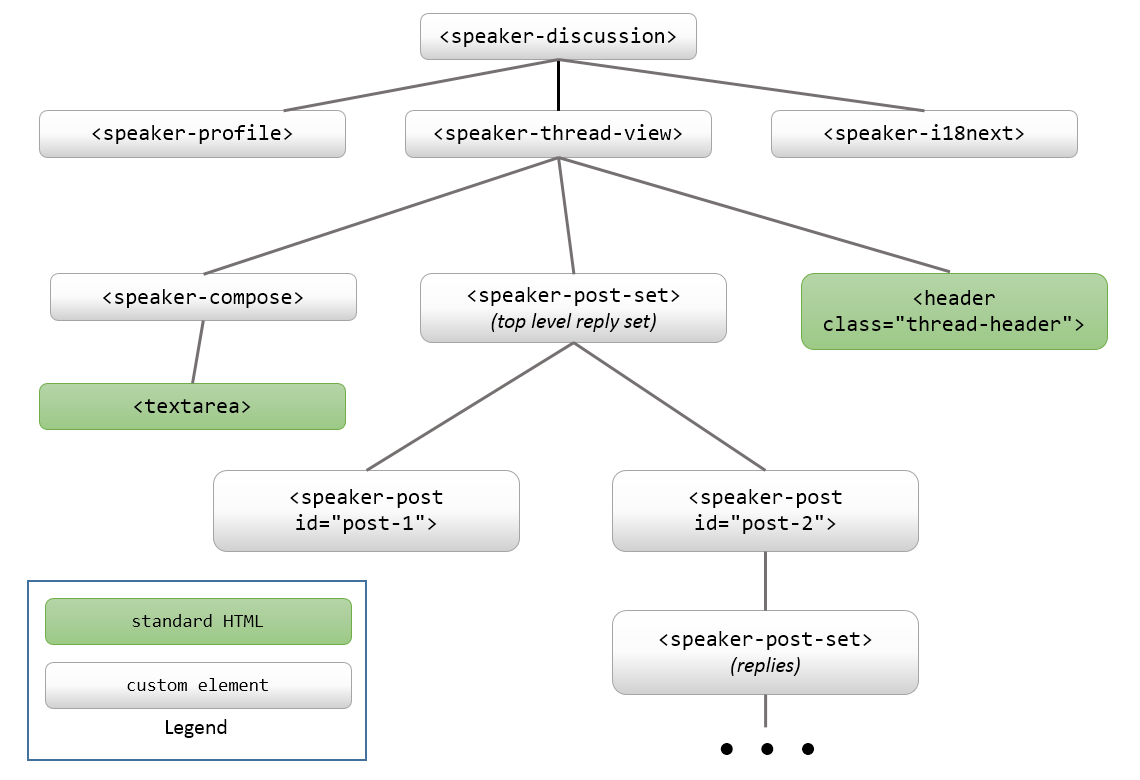
\includegraphics[width=6.2in]{images/components.png}}
	\caption{Speakur component hierarchy (partial).}
	\label{f:component_layout}
\end{figure}

Blah blah...


\subsection{Data Bindings and Events}
\label{sec:databindings}

\subsection{Data-Bound Templates}

\section{Security}
\label{sec:security}

\subsection{Authentication}

\subsection{Firebase Security Policy Rules}
\label{sec:fbsecurity}

\section{Internationalization}
\label{sec:i18n}

\subsection{Architecture}
\subsection{Libraries}

\section{Responsive Design}
\label{sec:responsive}

\subsection{Mobile Users}

\subsection{Accessibility}

\section{Publishing and Deployment}
\label{publishing}
